\chapter{序論}
\section{研究の背景と目的}
\subsection{AIの始まり}
AIの概念の始まりは,1950年にアラン・チューリングが提唱したチューリングテストである.\cite{ronbun1}
チューリングテストとは,男性、女性、質問者の3人でおこなわれ,目的は質問者がどちらが男性でどちらが女性かを当てるゲームである.会話は文字だけでおこない,男性は質問者を間違わせるように振舞い,逆に女性は質問者を助けるように振舞う.
このゲームの男性の代わりに機械がなり,質問者が二人の人間を相手にした時と同じくらいの間違いを,人間と機械のペアにも起こすことができれば,機械は知性を持っているとする.
また,チューリングテストを受ける機械はどんな技術を使っても良く,機械を作った人が、その機械の動作の仕様をきちんと説明できないようなものであってもかまわないということを認めている.
この概念が提唱されてから初めてチューリングテストに合格したのは,2014年にレディング大学で開催された「Turing Test 2014」で発表された,ウクライナ在住の13歳の少年が開発した「Eugene Goostman」というプログラムだった.
\begin{figure}[!ht]
    \begin{screen}
    \begin{center}
        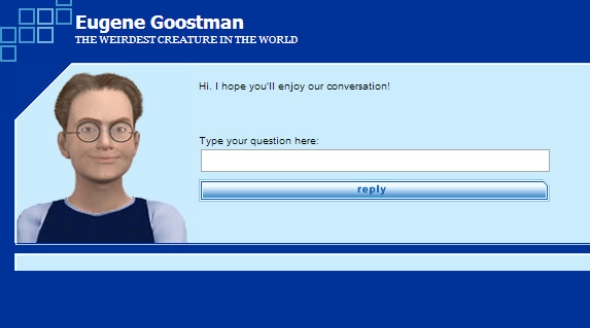
\includegraphics[scale=0.6, clip]{./img/Eugene_Goostman.jpg}
        \caption{チューリングテストを合格したEugeneGoostman\newline(引用:http://www.itmedia.co.jp/news/articles/1807/26/news014.html)}
        \label{fig:チューリングテストを合格したEugeneGoostman}
    \end{center}
\end{screen}
\end{figure}
\subsection{第1次AIブーム}
その後,次のAIブームは1950年代後半から1960年代に起きた.
この時代になり初めてAI(Artificial Intelligence,人工知能)という言葉がダートマス会議で用いられた.\\
この会議は1956年に米ニューハンプシャー州のダートマス大学で開催され,コンピュータ研究者たちの研究成果を発表し合う研究発表会である.\cite{webpage4}
この会議の発起人であるジョン・マッカーシー氏がAIという言葉をThe Dartmouth Summer Research Project on Artificial Intelligence\cite{ronbun2}の中で用いた.
また,この会議で初めての人工知能プログラムと言われる“Logic Theorist”と呼ばれる数学原理をコンピュータで証明するデモンストレーションが行われ,当時のコンピュータはせいぜい四則演算が限界だったため,これは画期的な成果といえた.\\
他にも,マサチューセッツ工科大学のジョセフ・ワイゼンバウム氏が1966年に作成した単純な自然言語処理プログラム「ELIZA」が発表された.
ただ,ELIZAはそのプログラムはパターン照合を適用しているため,パターンにない会話はできないため曖昧な事柄に対応できない.
また、人工知能の理解は文字列だけにしか及ばず、これを記号に結びつけることが出来ないという「シンボルグラウンティング問題」が指摘される.
例えば、「馬」と「縞(シマ)」、それぞれの概念を知っている人はシマウマ=「馬」+「シマ」だと理解できるが、人工知能にはそれができない、というものである。
\subsection{第2次AIブーム}
1980年代に入り,家庭にコンピュータが普及したことにより第二次ブームが発生しました.
「知識」(コンピューターが推論するために必要な様々な情報を、コンピューターが認識できる形で記述したもの)を与えることで人工知能(AI)が実用可能な水準に達し、
多数のエキスパートシステムとよばれる,専門分野の知識を取り込んだ上で推論することで、その分野の専門家のように振る舞うプログラムが生み出された。
日本では、政府による「第五世代コンピュータ」と名付けられた大型プロジェクトが推進された。
しかし、当時はコンピューターが必要な情報を自ら収集して蓄積することはできなかったため、必要となる全ての情報について、人がコンピューターにとって理解可能なように内容を記述する必要があり,
世にある膨大な情報全てを、コンピューターが理解できるように記述して用意することは困難なため、実際に活用可能な知識量は特定の領域の情報などに限定する必要があった。
こうした限界から、1995年頃からブームは衰えた。
\subsection{第3次AIブームの始まり}
第二次AIブームでのエキスパートシステムが壁にぶつかった問題として,日常世界には例外処理や矛盾したルールが非常に多く,知識を教え込む作業が非常に困難というのがありました.
これらを解決する手段として「機械学習」や「ディープラーニング」にてコンピュータが自らが学んでいくという手法が第二次AIブームの時代から研究されていましたが,実用化するためにはコンピュータの性能が追い付いていなかった.\\
しかし,2000年代に入り,コンピューターの小型化・性能向上に加えインターネットの普及,クラウドでの膨大なデータ管理が容易となったことで実現可能なレベルとなり,第三次AIブームが沸き起こりました.
2006年にはニューラルネットワークの代表的な研究者であるジェフリー・ヒントンらの研究チームが、制限ボルツマンマシンによるオートエンコーダの深層化に成功し、再び注目を集めるようになった。
この際、発表した論文から、これまでの多層ニューラルネットよりもさらに深いネットワーク構造を意味する、ディープネットワークの用語が定着した。
2011年にIBMワトソンがクイズ番組難解な質問と独特の解答方法で知られる人気クイズ番組「ジョパディ!」に出場した.
ワトソンが読み込んだ本や映画の脚本、百科事典などは合計100万冊。公平を期すため、インターネットには接続しておらず、"頭の中"の蓄積だけが頼りだ。
\begin{figure}[!ht]
    \begin{screen}
    \begin{center}
        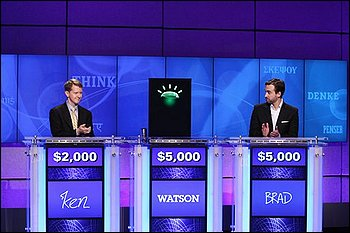
\includegraphics[scale=1.0, clip]{./img/Watson.jpg}
        \caption{クイズ番組に出演するWatson\newline(http://www.swift-web.org/cp-bin/blogn/index.php?e=1023)}
        \label{fig:クイズ番組に出演するWatson}
    \end{center}
\end{screen}
\end{figure}\\
このときまで、機械学習のほとんどは、ラベル付きデータの量に依存していた。
キャットペーパーにより、機械がラベルのない生データでも処理することができ、そしておそらく、人間が予備知識を持たないデータですら処理できることが示された。
\subsection{第3次AIブームの現在}
2014年にはAmazon.comからスマートスピーカと呼ばれる対話型の音声操作に対応したAIアシスタント機能を持つスピーカーであるAmazon Echoが発売され,その後GoogleやAmazon,IBMによって様々なスマートスピーカーが商品化された.
現在ではスマートフォンにもSiriというAIが搭載されるなどその存在は非常に身近になっており,その種類も非常に多岐にわたる.
\begin{figure}[!ht]
    \begin{screen}
    \begin{center}
        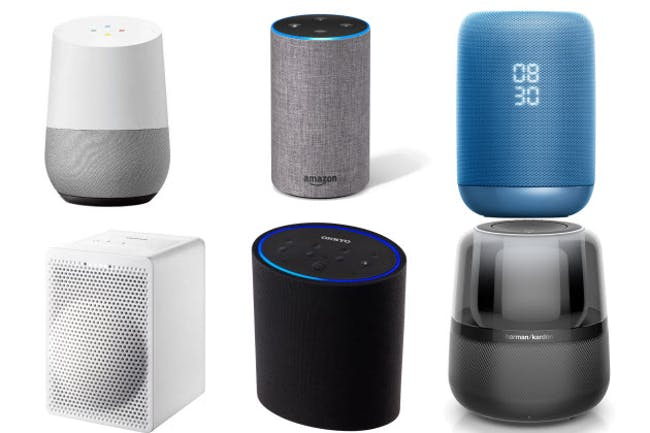
\includegraphics[scale=0.6, clip]{./img/smartspeaker_list.jpg}
        \caption{多種多様なスマートスピーカー}
        \label{fig:多種多様なスマートスピーカー}
    \end{center}
\end{screen}
\end{figure}\\
囲碁や将棋,チェスなどの競技においても,プロにAIが勝利するなどその精度は以前から高いが,そのAIは一つの競技でしか使用できない特化型人工知能(AGI)でありった.
しかし,英DeepMindが発表したAlphaZeroという様々なボードゲームに対応できる汎用性を持ったAIが発表され,汎用人工知能(GAI)の成長も著しい.\\
自然言語処理を用いた芸術の分野では,2012年にスタートした人工知能を使って小説を生成するプロジェクトが「星新一賞」の第一審査を通過した.\cite{webpage2}
また,絵画や音楽に関してもAIが作成した肖像画が米競売大手クリスティーズのオークションで43万2500ドル(約4900万円)で落札され,AIを用いて新しい作品を作るものが出回っている.\cite{webpage3}\\
\subsection{様々なAI楽曲作成サービス}
AIを用いた楽曲作成サービスはAmper Musicという「作成したい音楽ジャンル」と「曲の長さ」を指定すれば,AIがオリジナル曲を作曲してくれるサービスです. 作成した曲は,テンポを変えたり,楽器を追加したりと後からも編集できるようにもなっている.また,Jukedeck
本研究ではAIによる楽曲生成についての実証実験を行う.
Googole brainによって公開されているTensorflowのライブラリであるMagentaはAI Duet
そのライブラリを用いて学習データやノード数による楽曲の生成結果の違いを比較,検証し,AIによる楽曲制作が有用なものか調査する.\\
\section{本論文の構成}
本論文の構成は以下の通りである.\\
第1章では本論文の背景と目的について述べている.\\
第2章では本論文で利用する理論について述べている.\\
第3章では実験内容について述べている.\\
第4章では楽曲制作について述べている.\\
第5章ではAIを用いた楽曲制作についての本研究の結論について述べている.\\